\documentclass[sigconf]{webmedia}

\AtBeginDocument{
  \providecommand\BibTeX{{
    \normalfont B\kern-0.5em{\scshape i\kern-0.25em b}\kern-0.8em\TeX}}}

\settopmatter{printacmref=false, printfolios=false}

\proceedingsDetails [WTVDI'2026]{IX Workshop Futuro da TV Digital Interativa (WTVDI 2026). Anais Estendidos do XXXII Simpósio Brasileiro de Sistemas Multimídia e Web}{2026}{Lavras/MG, Brazil}
\ISSN{2596-1683}

\usepackage{tikz}
\usetikzlibrary{positioning,shapes,arrows,matrix,shapes.geometric,fit,calc}
\usepackage{subcaption}
\usepackage{listings}
\usepackage{stfloats}
\usepackage{booktabs}
\usepackage{array}
\usepackage{algorithm}
\usepackage{algpseudocode}

\lstset{
  basicstyle=\ttfamily\footnotesize,
  columns=fullflexible,
  keepspaces=true,
  breaklines=true,
  frame=single,
  showstringspaces=false
}

\begin{document}

\title{NCL Users API: \texttt{gingaf} support and new proposed user attribute for \texttt{<rule>}}

\author{Alan L. V. Guedes}
\email{a.guedes@reading.ac.uk}
\affiliation{%
  \institution{University of Reading}
  \country{UK}
}

\author{Paulo Victor Borges}
\orcid{0009-0002-3620-477X}
\email{paulo.victor.lima15@gmail.com}
\affiliation{%
  \institution{PUC-Rio}
  \country{Brazil}
}

\author{Daniel Moraes}
\orcid{0000-0003-2995-3115}
\email{danielmoraes@telemidia.puc-rio.br}
\affiliation{%
  \institution{PUC-Rio}
  \country{Brazil}
}

\author{Sergio Colcher}
\orcid{0000-0002-3476-8718}
\email{colcher@puc-rio.br}
\affiliation{%
  \institution{PUC-Rio}
  \country{Brazil}
}

\renewcommand{\shortauthors}{Guedes et al.}

\begin{abstract}
The SBTVD TV 3.0 specification proposes a paradigm shift for its middleware, Ginga, from traditional isolated single-viewer set-top box experiences toward multi-user personalized interactive environments. In this paper, we present the implementation of the \textbf{NCL Users API} in \texttt{gingaf}, an open-source cross-platform Ginga implementation. We demonstrate how \texttt{gingaf} handles dynamic user profile resolution, user settings property binding, and profile data initialization. Furthermore, we propose an extension to the NCL Users API to address the verbosity of causal link assessments by extending NCL's \texttt{<rule>} element with a \texttt{user} attribute. This attribute allows conditional presentation using \texttt{<switch>} elements. Finally, we verify compliance and validate our implementation in multi-user content scenarios.
\end{abstract}

\keywords{Digital Television, TV 3.0, Ginga, NCL}

\begin{teaserfigure}
  \centering
  \begin{subfigure}[b]{0.48\textwidth}
    \centering
    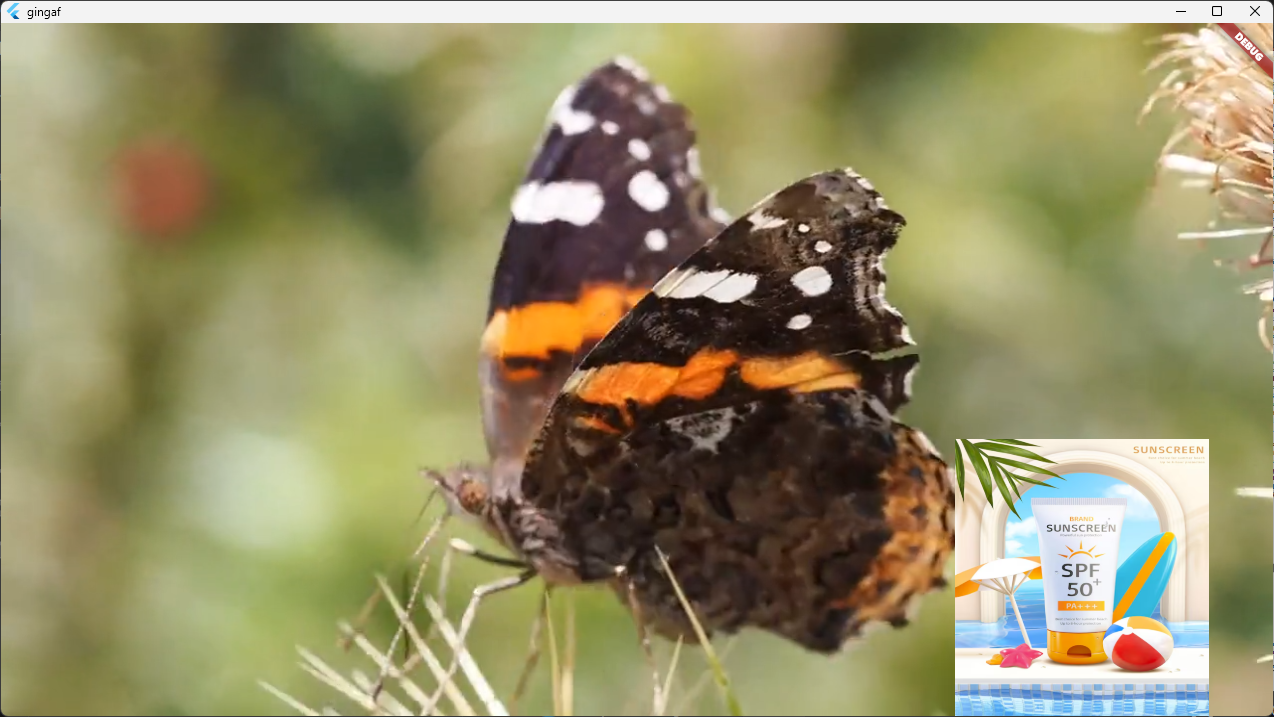
\includegraphics[width=\textwidth]{assets/image1.png}
    \caption{Scenario without adult male user (displays general advertisement).}
    \label{fig:teaser_no_adult}
  \end{subfigure}
  \hfill
  \begin{subfigure}[b]{0.48\textwidth}
    \centering
    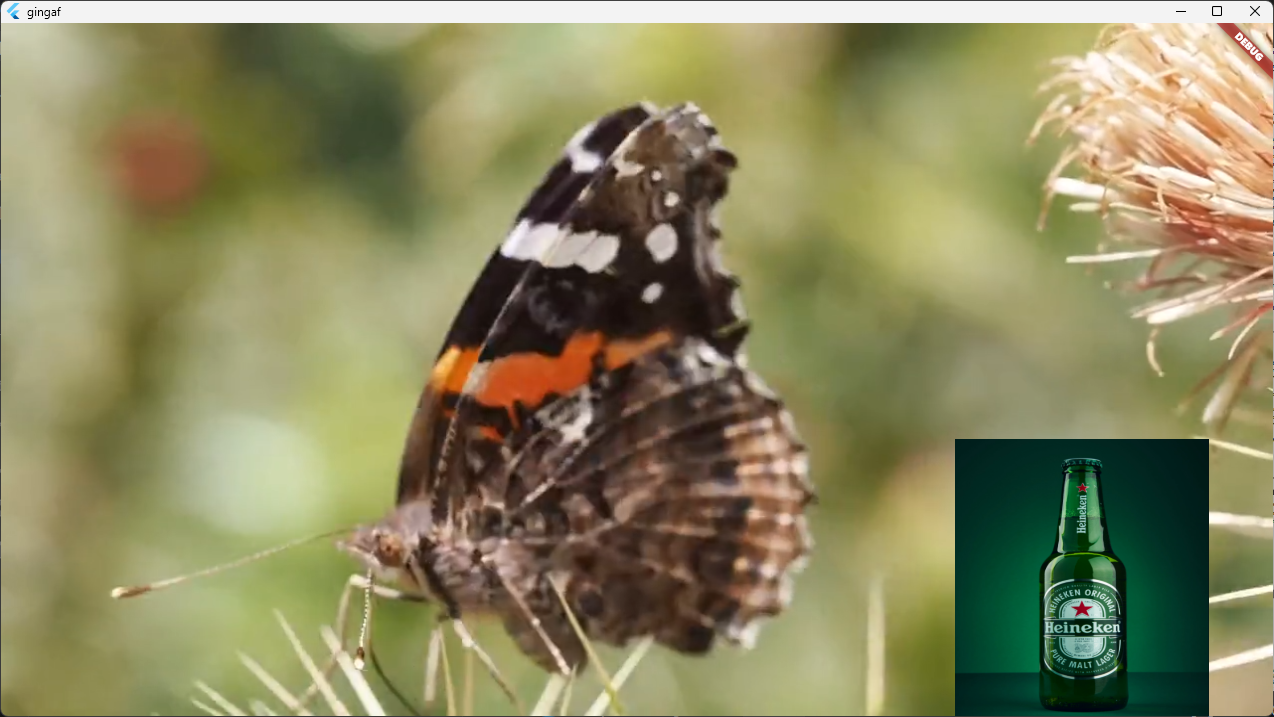
\includegraphics[width=\textwidth]{assets/image2.png}
    \caption{Scenario with adult male user (displays male advertisement).}
    \label{fig:teaser_with_adult}
  \end{subfigure}
  \caption{NCL application running in two multi-user scenarios.}
  \label{fig:teaser}
\end{teaserfigure}

\maketitle

\section{Introduction}
\label{sec:intro}
Digital television systems worldwide are undergoing a fundamental transformation toward TV 3.0—a next-generation architecture characterized by advanced audio-visual compression, IP-based broadcast-broadband convergence, multi-screen companion device integration, and personalized user experiences~\cite{santos2026overview}. In modern domestic environments, multiple family members frequently watch shared main-screen broadcasts while simultaneously interacting with personal companion devices such as smartphones, tablets, or secondary displays~\cite{souza2020ncl360}. Traditional interactive middleware architectures, including early Ginga-NCL specifications~\cite{soares2010ginga, ITU_H761}, evaluated application execution context through global system variables (e.g., \texttt{system.language} or \texttt{system.caption}). While suitable for single-user set-top box setups, global state models fail in concurrent multi-viewer living room scenarios where distinct individuals require personalized accessibility options, localized language tracks, customized focus navigation, or targeted commercial content on secondary screens.

To overcome these structural limitations, the Brazilian Digital Terrestrial Television (SBTVD) Forum standardized the TV 3.0 specification~\cite{abnt_15608_4}, establishing the \textit{NCL Users API}. This standard defines explicit primitives for managing concurrent user profiles and binding causal hypermedia links to dynamic user properties. This paper introduces an open-source implementation of the NCL Users API in the cross-platform Ginga implementation \texttt{gingaf}~\cite{gingaf2026}. Built upon the headless logic package \texttt{ncl\_doc} and Flutter presentation layers, \texttt{gingaf} delivers centralized profile management, reactive property evaluation, and multi-device focus routing.

To support reproducibility, the source code, unit tests, and demonstration videos are available at \textcolor{ACMDarkBlue}{\url{https://github.com/ginga-org-br/gingaf}}.

The remainder of this paper is structured as follows. Section~\ref{sec:background} provides a background on the TV 3.0 Multiuser API. Section~\ref{sec:multiuser} describes the design and implementation of multi-user support in \texttt{gingaf}. Section~\ref{sec:rule_proposal} discusses the proposed user attribute for \texttt{<rule>}. Finally, Section~\ref{sec:remarks} presents our final remarks and outlines future work.

\section{Background on TV 3.0 Multiuser API}
\label{sec:background}

Prior to TV 3.0, user settings were represented as key-value pairs stored in the global \texttt{system} node, meaning that modifying a global attribute affected all connected viewers unconditionally. To address these multi-user living room contexts, the TV 3.0 standard~\cite{abnt_15608_4} introduces new XML elements into the NCL schema to support multi-user profiles and dynamic settings.

First, the {\small\textbf{\texttt{<userProfile>}}} element, grouped within the \texttt{<userBase>} container (line~\ref{line:userBase} of Listing~\ref{lst:ncl}), represents individual user profiles. It supports local attribute initialization or remote profile queries via the \texttt{src} attribute, as shown on line~\ref{line:userProfile} of Listing~\ref{lst:ncl}. The \texttt{src} attribute allows dynamic resolution of user profile data from external JSON endpoints, as shown in Listing~\ref{lst:adult_query_json}.

Second, a {\small\textbf{\texttt{<media type="application/x-ncl-user-settings">}}} \newline element (or a settings node via the \texttt{<settings>} element) binds these user profile attributes to NCL variables. As shown on line~\ref{line:settings} of Listing~\ref{lst:ncl}, it maps attributes using the \texttt{pAdult} alias, which acts as a dynamic reference pointing to the active viewer interacting with the application.

Third, causal connectors defined in the \texttt{<connectorBase>} (line~\ref{line:connectorBase} of Listing~\ref{lst:ncl}) evaluate user properties using assessment statements. The \texttt{onBeginTestVarStart} connector (line~\ref{line:causalConnector}) tests if a node property variable equals a parameter value \texttt{\$value} upon element start. As shown on lines~\ref{line:linkMale} and~\ref{line:linkGeneral}, two causal links bind the \texttt{gender} property of \texttt{uSettings} and the area anchor at 2 seconds (\texttt{aSec2}, line~\ref{line:area}) of \texttt{mVideo}: the first evaluates if \texttt{gender} equals \texttt{"male"} to start \texttt{mMaleAd}, while the second evaluates if \texttt{gender} equals \texttt{"female"} to start \texttt{mGeneralAd}.

This enables single-device broadcast receivers to evaluate targeted advertisement links (e.g., selecting male-targeted commercial breaks when \texttt{gender} = ``male'') synchronously upon document initialization. The \texttt{Users} singleton maintains the registry of active users. When a query is run against these users, the system parses the query schema from the profile source, as defined in Listing~\ref{lst:adult_query_json}.

\begin{lstlisting}[language=XML, escapeinside={(*}{*)}, caption={video.ncl source code}, basicstyle=\footnotesize\ttfamily, frame=single, breaklines=true, aboveskip=1mm, belowskip=1mm, captionpos=b, numbers=left, label={lst:ncl}]
<ncl>
<head>
<regionBase>
  <region id="rgAd" left="75%" top="75%" width="20%" height="20%"/>
</regionBase>
<descriptorBase>
  <descriptor id="dAd" region="rgAd"/>
</descriptorBase>
<connectorBase> (*\label{line:connectorBase}*)
  <causalConnector id="onBeginTestVarStart"> (*\label{line:causalConnector}*)
    <compoundCondition operator="and">
      <simpleCondition role="onBegin"/>
      <assessmentStatement comparator="eq">
        <attributeAssessment role="var" attributeType="nodeProperty" eventType="attribution"/>
        <valueAssessment value="$value"/>
      </assessmentStatement>
    </compoundCondition>
    <simpleAction role="start"/>
  </causalConnector>
</connectorBase>
<userBase> (*\label{line:userBase}*)
  <userProfile id="pAdult" src="adult_query.json" max="1"/> (*\label{line:userProfile}*)
</userBase>
</head>
<body>
  <settings id="uSettings" type="application/x-ncl-user-settings" user="pAdult"> (*\label{line:settings}*)
    <property name="gender"/>
  </settings>
  <port id="pMain" component="mVideo"/>
  <media id="mVideo" src="video.mp4">
    <area id="aSec2" begin="2s"/> (*\label{line:area}*)
  </media>
  <media id="mMaleAd" src="ad_male.png" descriptor="dAd"/>
  <media id="mGeneralAd" src="ad_general.png" descriptor="dAd"/>
  <link xconnector="onBeginTestVarStart"> (*\label{line:linkMale}*)
    <bind role="onBegin" component="mVideo" interface="aSec2"/>
    <bind role="var" component="uSettings" interface="gender"/>
    <bindParam name="value" value="male"/>
    <bind role="start" component="mMaleAd"/>
  </link>
  <link xconnector="onBeginTestVarStart"> (*\label{line:linkGeneral}*)
    <bind role="onBegin" component="mVideo" interface="aSec2"/>
    <bind role="var" component="uSettings" interface="gender"/>
    <bindParam name="value" value="female"/>
    <bind role="start" component="mGeneralAd"/>
  </link>
</body>
</ncl>
\end{lstlisting}

\begin{lstlisting}[caption={\texttt{adult\_query.json}}, basicstyle=\footnotesize\ttfamily, label={lst:adult_query_json}]
{"attribute": "age", "comparator": "gte", "value": "18"}
\end{lstlisting}

\section{\texttt{gingaf} Multi-user Support}
\label{sec:multiuser}

\texttt{gingaf} is a decoupled open-source digital television middleware player executing NCL applications via the headless package \texttt{ncl\_doc} and a Flutter rendering engine. To illustrate this behavior, we describe two scenarios running the previously detailed NCL application.

\texttt{gingaf} saves user attributes in \texttt{NCLUserData}, which maintains a key-value map for variables. Initial user profiles can be injected into \texttt{gingaf} via the \texttt{usersDataSrc} configuration parameter, which should contain the path to a JSON file with a list of users and their properties. Algorithm~\ref{alg:multiuser_flow} details the parsing and profile matching process given an NCL document $D$ and user dataset $Users$.

\begin{algorithm}
\caption{User Profile Properties Parsing}
\label{alg:multiuser_flow}
\renewcommand{\algorithmicrequire}{\textbf{input:}}
\begin{algorithmic}[1]
\Require NCLDocument $D$, usersData $Users$
\For{\raggedright each \texttt{<media>} $m \in D$ of type \texttt{application/x-ncl-user-settings}}
    \State $p \gets \text{loadUserProfileQuery}(m.\text{user})$
    \State $u \gets \text{matchProfile}(Users, p)$
    \State $m.\text{loadPropertiesFromUser}(u)$
\EndFor
\State Execute NCLDocument $D$
\end{algorithmic}
\end{algorithm}

To illustrate multi-user support in \texttt{gingaf}, we execute the application from Listing~\ref{lst:ncl} for two multi-user scenarios.

The first is a \textbf{scenario without a male user} (Figure~\ref{fig:teaser_no_adult}), using the user profile definitions described in Listing~\ref{lst:users_no_adult_json}. It has two female users: one adult and one underage.

\begin{lstlisting}[caption={\texttt{users\_data\_no\_adult\_male.json}}, basicstyle=\footnotesize\ttfamily, label={lst:users_no_adult_json}]
[
  {"id": "u2", "name": "Alice", "gender": "female", "age": 30},
  {"id": "u3", "name": "Kid", "gender": "female", "age": 10}
]
\end{lstlisting}

The second is a \textbf{scenario with a male user} (Figure~\ref{fig:teaser_with_adult}), using the user profile definitions described in Listing~\ref{lst:users_with_adult_json}. It has one adult male user and one underage female user. In this case, the adult profile query resolves to the male user (\texttt{Bob}), triggering the targeted advertisement.

\begin{lstlisting}[caption={\texttt{users\_data\_with\_adult\_male.json}}, basicstyle=\footnotesize\ttfamily, label={lst:users_with_adult_json}]
[
  {"id": "u1", "name": "Bob", "gender": "male", "age": 30},
  {"id": "u3", "name": "Kid", "gender": "female", "age": 10}
]
\end{lstlisting}

\section{Proposed User Attribute for \texttt{<rule>}}
\label{sec:rule_proposal}

To avoid the verbosity of explicit \texttt{<valueAssessment>} statements within causal links, NCL authors can alternatively handle conditional media presentation using the \texttt{<switch>} element. However, as specified in Section 7.2.9 (Presentation control functionality) of ABNT NBR 15606-2:2023~\cite{abnt_15606_2_2023}, \texttt{<rule>} elements defined within the \texttt{<ruleBase>} implicitly target properties from global system variables (e.g., \texttt{system.language}):

\begin{lstlisting}[language=XML, caption={Standard \texttt{<rule>} definition targeting global system variables.}, basicstyle=\footnotesize\ttfamily, frame=single, breaklines=true, aboveskip=1mm, belowskip=1mm, captionpos=b]
<ruleBase>
  <rule id="en" var="system.language" value="en" comparator="eq"/>
</ruleBase>
\end{lstlisting}

To support multi-user living room contexts without requiring verbose link assessments, we propose extending the \texttt{<rule>} element with an explicit \texttt{user} attribute (e.g., \texttt{user="pAdult"}). This parameter specifies which user settings node or profile is being evaluated during rule resolution. Listing~\ref{lst:ncl_bindrule} demonstrates this proposed syntax within an NCL application \texttt{<switch>}.

\begin{lstlisting}[language=XML, escapeinside={(*}{*)}, caption={Proposed NCL application using \texttt{<switch>} and \texttt{user} parameter at \texttt{<rule>}.}, basicstyle=\footnotesize\ttfamily, frame=single, breaklines=true, aboveskip=1mm, belowskip=1mm, captionpos=b, numbers=left, label={lst:ncl_bindrule}]
<ncl>
<head>
<regionBase>
  <region id="rgAd" left="75%" top="75%" width="20%" height="20%"/>
</regionBase>
<descriptorBase>
  <descriptor id="dAd" region="rgAd"/>
</descriptorBase>
<userBase>
  <userProfile id="pAdult" src="adult_query.json" max="1"/>
</userBase>
<ruleBase>
  <rule id="rMale" user="pAdult" var="gender" comparator="eq" value="male"/>
</ruleBase>
</head>
<body>
  <settings id="uSettings" type="application/x-ncl-user-settings" user="pAdult">
    <property name="gender"/>
  </settings>
  <port id="pMain" component="swAd"/>
  <switch id="swAd">
    <bindRule rule="rMale" constituent="mMaleAd"/>
    <defaultComponent component="mGeneralAd"/>
    <media id="mMaleAd" src="ad_male.png" descriptor="dAd"/>
    <media id="mGeneralAd" src="ad_general.png" descriptor="dAd"/>
  </switch>
</body>
</ncl>
\end{lstlisting}

\section{Final Remarks}
\label{sec:remarks}

We presented \texttt{gingaf}, a complete open-source implementation of the NCL Users API conforming to TV 3.0 specifications. Future work will expand \texttt{gingaf} to incorporate user profile authentication with companion devices.

\bibliographystyle{ACM-Reference-Format}
\bibliography{references}

\end{document}